\documentclass[a4paper]{article}
\usepackage[brazilian]{babel}
\usepackage{times}
\usepackage[hmargin=3cm,vmargin=3cm,bmargin=4cm]{geometry}
\usepackage[utf8]{inputenc}
\usepackage{graphicx}
\usepackage{gensymb}
\usepackage{siunitx}
\usepackage{listings}
\usepackage{verbatim}
\usepackage{bigints}
\usepackage{breqn}
\usepackage{titling}
\usepackage[colorinlistoftodos]{todonotes}
\usepackage[section]{placeins}
\usepackage{amssymb}
\usepackage{ifpdf}
%\usepackage[unicode]{hyperref}
\usepackage{hyperref}
\usepackage{url}
\usepackage[T1]{fontenc}
\usepackage{subcaption}
\usepackage{booktabs}
\usepackage{tikz}
\usepackage[RPvoltages]{circuitikz}
%\usepackage{floatrow}
%\floatsetup[table]{capposition=top}
\usepackage{textcomp}
%\usepackage{textgreek}
\usepackage{graphicx}
\usepackage{color}
%\usepackage{floatrow}
\usepackage{caption}
\usepackage{cleveref}
\usepackage{indentfirst}
\definecolor{mygreen}{RGB}{28,172,0} % color values Red, Green, Blue
\definecolor{mylilas}{RGB}{170,55,241}
\usepackage{varwidth}
\usepackage{amsmath}
\usepackage{float}
\usepackage{subfigure}



\hypersetup{
  colorlinks   = true, %Colours links instead of ugly boxes
  urlcolor     = blue, %Colour for external hyperlinks
  linkcolor    = black, %Colour of internal links
  citecolor   = black    %Colour of citations
}

\begin{document}

\begin{titlepage}
\begin{center}
\vspace{25mm}
\rule[0.5ex]{\linewidth}{2pt}\vspace*{-\baselineskip}\vspace*{3.2pt}
\rule[0.5ex]{\linewidth}{1pt}\\[\baselineskip]
{\huge\textbf{Projeto Final\\Controle LQR de um pêndulo invertido}}\\[4mm]
{\Large \textit{ES728 - Controle Avançado de Sistemas}}\\
\rule[0.5ex]{\linewidth}{1pt}\vspace*{-\baselineskip}\vspace{4pt}
\rule[0.5ex]{\linewidth}{2pt}\\
\vspace{05mm}
{\large Autores}\\
\vspace{5mm}
{\large
\textsc{Carlos Augusto Jardim Chiarelli  \hfill RA: 165685\\}
\textsc{Lucas Belucci  \hfill RA: 172593\\}
}
\vspace{30mm}
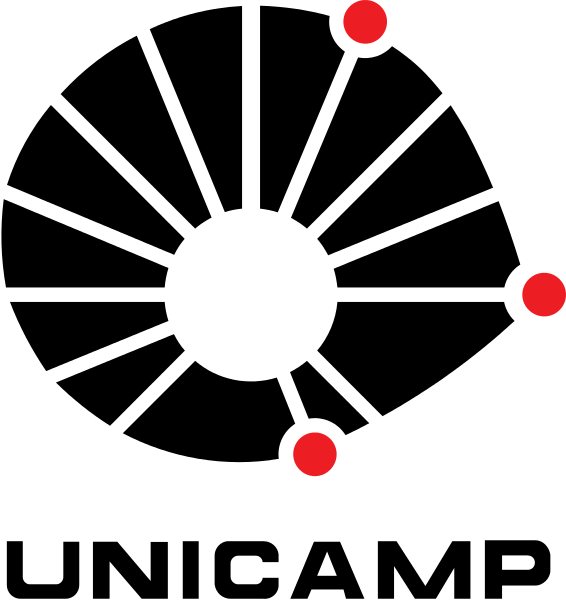
\includegraphics[scale=0.3]{UNICAMP.png}\\
\vspace{6mm}
{\large Faculdade de Engenharia Mecânica\\
\textsc{Universidade Estadual de Campinas}}\\
\vspace{25mm}
{\large\textsc{Campinas, Fevereiro de 2021}}
\vspace{12mm}
\end{center}

\end{titlepage}

\hypersetup{linkbordercolor=black}

\begin{center}
\tableofcontents
\end{center}
\newpage

\section{Projeto}
\begin{figure}[h]
\subfigure[Modelo pêndulo invertido]{
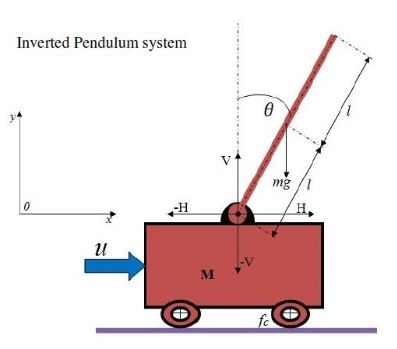
\includegraphics[width=8cm,height=8cm]{Modelo.JPG}}
\qquad 
\qquad
\subfigure[]{
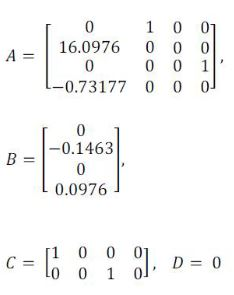
\includegraphics[width=5cm,height=5cm]{Matriz.JPG}}
\end{figure}

\subsection{Primeira parte(vetor de estado conhecido)}
\begin{enumerate}
    \item \textbf{Projetar um controlador LQR para o controle do pêndulo invertido, usando o mesmo modelo apresentado na seção “IV –Design of LQR”do artigo anexo.}
    \item \textbf{Repetir as simulações das figuras 2,3,4,5 desse artigo.}
    \end{enumerate}
    
Para a obtenção do controlador LQR, iremos utilizar a ferramenta Matlab. E para isso precisamos definir as matriz A, B, C e D como informadas no enunciado. Portanto:\\
\newline
A = $ \begin{pmatrix} 
0 & 1 & 0 & 0 \\ 16.0976 & 0 & 0 & 0 \\ 0 & 0 & 0 & 1 \\ -0.73177 & 0 & 0 & 0\\
\end{pmatrix}$ \qquad \qquad
B = $ \begin{pmatrix}
0 \\ -0.1463 \\ 0 \\ 0.0976\\
\end{pmatrix}$\\
\newline
\newline
C = $\begin{pmatrix}
1 & 0 & 0 & 0 \\ 0 & 0 & 1 & 0\\
\end{pmatrix}$ \qquad \qquad \qquad \qquad         D = $\begin{pmatrix}
0
\end{pmatrix}$\\
\newline
\newline
Como queremos encontrar apenas os valores de ganho para as saídas conhecidas e com o mesmo peso em relação ao controle, iremos assumir:\\
\(Q = C^{T}*C\)\\
\newline
Q = $\begin{pmatrix}
     1 & 0 & 0 &  0\\
     0 & 0 & 0 & 0\\
     0 & 0 & 1 & 0\\
     0 & 0 & 0 & 0\\
\end{pmatrix}$
\newline
\newline
\newline
R = 1\\
Depois disso podemos utilizar o comando \textit{care} do matlab então:
\newline
[P,L,K] = care(A,B,Q,R)\\
\newline
\newline
P = \(1*10^{3}\)$\begin{pmatrix}
     7.4681 & 1.8743 & 0.0612 &  0.3019\\
     1.8743 & 0.4705 & 0.0158 & 0.0780\\
     0.0612 & 0.0158 & 0.0052 & 0.0135\\
     0.3019 & 0.0780 & 0.0135 & 0.0637\\
\end{pmatrix}$
\newline
\newline
\newline
L = $\begin{pmatrix}
     -4.0122 + 0.0183i\\
     -4.0122 - 0.0183i\\
     -0.2133 + 0.2132i\\
     -0.2133 - 0.2132i\\
\end{pmatrix}$
\newline
\newline
\newline
K = $\begin{pmatrix}
     -244.7533 & -61.2266 & -1.00 & - 5.1889\\
\end{pmatrix}$
\newline
\newline
Com isso conseguimos encontrar os valores dos autovalores e dos ganhos para o controlador em malha fechada.Porém dessa maneira também conseguimos obter diretamente os valores do ganho L do observador. Outra maneira de obtermos os valores do ganho K do controlador é através do comando direto \textit{lqr}, dessa maneira, teremos:\\
K = lqr(A,B,Q,R)\\
Com os valores dos ganhos, definimos os estados, sendo Ac em malha fechada e encontramos os gráficos solicitados de resposta ao impulso, resposta ao impulso com condições iniciais diferentes de zero e finalmente resposta ao impulso com presença de distúrbio, logo:\\
Ac = [(A-B*K)]\\
Bc = [B]\\
Cc = [C]\\
Dc = [D]\\
\newline
sys = ss(Ac,Bc,Cc,Dc)\\
\newline
\newline
Ac = $\begin{pmatrix}
     0 & 1.00 & 0 &  0\\
     -19.7098 & -8.9574 & -0.1463 & -0.7591\\
     0 & 0 & 0 & 1.0\\
     23.1562 & 5.9757 & 0.0.976 & 0.5064\\
\end{pmatrix}$
\newline
\newline
\begin{figure}[!htb]
    \centering
    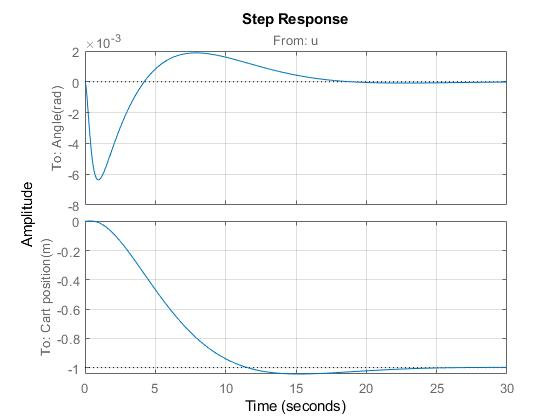
\includegraphics[scale = 0.6]{StepResponse_LQR.jpg}
    \caption{Step Response LQR}
\end{figure}
\newpage
\begin{figure}[!htb]
    \centering
    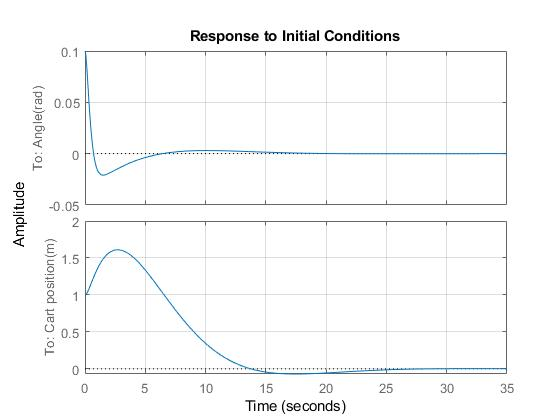
\includegraphics[scale = 0.6]{StepResponseCI_LQR.jpg}
    \caption{Step Response LQR with CI}
\end{figure}
\begin{figure}[!htb]
    \centering
    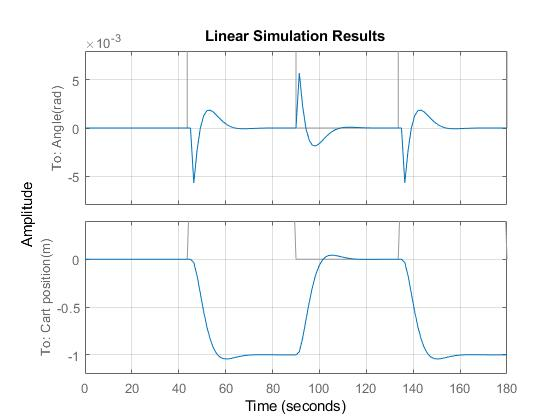
\includegraphics[scale = 0.6]{StepResponseDisturb_LQR.jpg}
    \caption{Step Response with step disturbance}
\end{figure}
\newpage
















\textbf{O “método” deve ser utilizado para que potência e torque máximos declarados pela Honda (motor R20Z1), Audi (motor A4 1.8) ou pela Porsche (968) (ou por qualquer outro fabricante, para qualquer modelo de motor), sejam estimados com a melhor precisão possível. Parâmetros geométricos do motor são apresentados na Tabela 1, bem como seus resultados operacionais. Os resultados conhecidos são para operação com gasolina pura.}
\begin{table}[ht]
    \centering
    \begin{tabular}{|c|c|c|c|c|}
        \hline
    Parâmetro &	Honda R20Z1 & Audi A4 1.8 &	Porsche 968 &	Unidade\\
    \hline
    Número de cilindros &	4 &	4 &	4 &	---\\
    \hline
    \# de tempos (de operação) &	4 &	4 &	4 &	---\\
    \hline
    Cilindrada (declarada) & 2.000 & 1.800 & 2.990 & cm3\\
    \hline
    Taxa de compressão & 11,1:1 & 10,3:1 & 11,0:1 & ---\\
    \hline
    Curso dos pistões &	96,9 & 86,4 & 88,0 & mm\\
    \hline
    Diâmetro dos pistões &	81,0 &	81,0 &	104,0 &	mm\\
    \hline
    Potência máxima & 155 @ 6.000 rpm &	123 @ 5.800 rpm & 237 @ 6.200 rpm &	HP\\
    \hline
    Torque máximo &	190 @ 4.500 rpm & 173 @ 3.950 rpm &	306 @ 4.100 rpm	& N.m\\
    \hline
    Velocidade máxima &	190 & 202 & 253 & km/h\\
    \hline
    \end{tabular}
    \caption{Parâmetros conhecidos dos dois motores (e dos veículos) e resultados para operação a plena carga}
\end{table}

\vspace{3mm}

\textbf{1 - Para o motor escolhido, ajuste o procedimento para que os resultados de potência efetiva e torque máximos sejam adequados em relação aos parâmetros de desempenho divulgados pelos fabricante.}
\vspace{2mm}

\textbf{2 - Compare a temperatura máxima operacional do ciclo nos dois pontos em que o modelo foi ajustado (i.e. para a reproduzir potência efetiva e torque máximos).}
\vspace{2mm}

\textbf{3 - Compare os parâmetros operacionais listados a seguir para os dois pontos em que o modelo foi ajustado (potência e torque máximos): rendimento mecânico, rendimento volumétrico, rendimento indicado, rendimento térmico e CEC.}
\vspace{2mm}

\textbf{4 - Qual o efeito das condições ambiente (temperatura e pressão atmosférica) (i.e. varie no modelo ambos parâmetros) sobre os seguintes parâmetros de desempenho: potência efetiva, torque, rendimento térmico e CEC?}
\vspace{2mm}

\textbf{5 - O procedimento disponível permite a análise do impacto do combustível usado. O ajuste disponível é para a consideração de operação com gasolina pura (do ponto de vista químico, é suposto octano). Qual o impacto da operação com etanol puro?\\ Simplificadamente, suponha que os parâmetros para etanol são os mesmos da operação com gasolina, e compare os resultados dos parâmetros a seguir: potência efetiva, torque, rendimento térmico, CEC e fluxo de combustível. Em um motor flex-fuel, quais parâmetros são ajustados quando a operação passa de etanol para gasolina, e vice versa? Nesses motores, no Brasil, qual dispositivo permite a identificação do combustível em uso?}
\vspace{2mm}

\textbf{6 - Qual o impacto do parâmetro “ALFA” (célula c17 na planilha) sobre os seguintes resultados de desempenho: potência efetiva, torque, rendimento térmico e CEC? Há uma situação em que o motor tem maior potência, e uma em que é mais eficiente? Caso a resposta seja afirmativa, em que condição o motor deve operar em trânsito normal? Diz-se que quando o motor é instantaneamente acelerado, o condutor quer ter maior torque. Assim, como é feito o controle para que o motor tenha resposta imediata, quando é acelerado?}
\vspace{2mm}

\textbf{7 - Observe o estado termodinâmico dos gases no fim do processo de expansão. O que sugere esse estado termodinâmico? É possível aproveitar a energia associada? Como?}
\vspace{2mm}

\textbf{8 - Na regulação Europeia, os veículos leves devem emitir menos de 180 gCO2/km rodado, e essas emissões deverão estar abaixo de 120-130 gCO2/km rodado em poucos anos. A partir dos resultados do procedimento disponível, qual a estimativa de emissões de CO2 (em gCO2/km) quando da operação do veículo em velocidade máxima, com gasolina pura?}
\vspace{5mm}

\subsection{Obtendo valores mais próximos aos do fornecedor}
Escolhendo o motor do Audi A4 1.8, portanto utilizando os parâmetros fornecidos na Tabela 1 e variando os valores na planilha excel fornecida, conseguimos obter valores mais próximos aos fornecidos pelas montadoras. Logo teremos:

\begin{table}[ht]
    \centering
    \begin{tabular}{|c|c|c|c|c|}
        \hline
    Parâmetro &	Audi A4 1.8 & Valor obtido & Erro & Unidade\\
    \hline
    Cilindrada (declarada) & 1.800 & 1781 & -1.06 \% & \(cm^{3}\)\\
    \hline
    Potência efetiva (Arques) & 123 & 123.97 & 0.79 \% & HP\\
    \hline
    Potência efetiva (ABNT) & 123 & 118,12 & -3.97 \% & HP\\
    \hline
    Potência efetiva (Khovakh) & 123 & 113.75 & -7,52 \% & HP\\
    \hline
    Torque correspondente &	151.5 & 150.02 & -0.98 \% & N.m\\
    \hline
    \end{tabular}
    \caption{Parâmetros ajustados para obtenção da potência efetiva para o motor em plena carga}
\end{table}

Portanto vemos que o método de Arques obtém os valores mais aproximados em relação a potência efetiva. Para obtermos o valor de torque máximo indicado, utilizamos os valores de torque máximo = 173N.m, rotação = 3950 rpm  e potência = 72.5kW, valores obtidos na primeira referência indicada no final do trabalho, ajustando os valores da tabela novamente encontramos:

\begin{table}[ht]
    \centering
    \begin{tabular}{|c|c|c|c|c|}
        \hline
    Parâmetro &	Audi A4 1.8 & Valor obtido & Erro & Unidade\\
    \hline
    Cilindrada (declarada) & 1.800 & 1781 & -1.06 \% & \(cm^{3}\)\\
    \hline
    Potência efetiva (Arques) & 97.1 & 96.99 & -0.11 \% & HP\\
    \hline
    Potência efetiva (ABNT) & 97.1 & 92.21 & -5.04 \% & HP\\
    \hline
    Potência efetiva (Khovakh) & 97.1 & 91.09 & -6.19 \% & HP\\
    \hline
    Torque máximo &	173 & 172.36 & -0.37 \% & N.m\\
    \hline
    \end{tabular}
    \caption{Parâmetros ajustados para a obtenção do torque máximo com o motor em plena carga}
\end{table}

Nesse caso vemos que o método de Arques continua a indicar um menor desvio para a potência efetiva. E observamos que conforme era esperado para a obtenção de um torque máximo adequado é necessário uma rotação diferente da fornecida para uma potência máxima, assim como pode ser observado em curvas características de torque x rotação.

\subsection{Temperatura máxima}
Comparando a temperatura máxima operacional para a situação de potência máxima e para a situação de torque máximo, teremos:
\begin{table}[!htb]
    \centering
    \begin{tabular}{|c|c|}
    \hline
     & Valor obtido\\
    \hline
    Temperatura admissão & 321.76 K\\
    \hline
    Temperatura máxima & 2639.65 K\\
    \hline
    Potência efetiva (Arques) & 123.97 HP\\
    \hline
    Potência efetiva (ABNT) & 118.12 HP\\
    \hline
    Potência efetiva (Khovakh) & 113.75 HP\\
    \hline
    \end{tabular}
    \caption{Para potência efetiva máxima}
\end{table}
\newpage
\begin{table}[!htb]
    \centering
    \begin{tabular}{|c|c|}
    \hline
    & Valor obtido\\
    \hline
    Temperatura admissão & 320.58 K\\
    \hline
    Temperatura máxima & 2630.42 K\\
    \hline
    Potência efetiva (Arques) & 96.99 HP\\
    \hline
    Potência efetiva (ABNT) & 92.21 HP\\
    \hline
    Potência efetiva (Khovakh) & 91.09 HP\\
    \hline
    \end{tabular}
    \caption{Para torque máximo}
\end{table}
Apesar da diferença de alguns parâmetros para obtermos potência máxima e torque máximo, ambos irão ocorrer quase a mesma temperatura na admissão, porém observamos que há uma diferença de aproximadamente 9 graus na temperatura máxima (T3), aumentando a potência fornecida.

\subsection{Parâmetros adicionais}
Observando os parâmetros adicionais teremos para a situação de potência efetiva máxima e de torque máximo a seguinte variação em relação ao modelo inicial.
\begin{table}[!ht]
    \centering
    \begin{tabular}{|c|c|c|c|}
    \hline
    & Valor (Pot. max.) & Valor ( Torq. max.) & Desvio\\
    \hline
    Temperatura máxima & 2639.65 K &  2630.42 K & -0.35 \% \\
    \hline
    Rendimento mecânico & 82.7 \% & 88.9 \% & 6.97 \%\\
    \hline
    Rendimento volumêtrico & 90.9 \% & 92.8 \%  & 2.05 \%\\
    \hline
    Rendimento indicado & 36.3 \% & 38 \% & 4.47 \%\\
    \hline
    Rendimento térmico & 27.3 \% & 31.4 \% & 13.06 \%\\
    \hline
    CEC & 303.2 g*kW/h & 263.7 g*kW/h & -14.98 \%\\
    \hline
    Consumo combustível & 7.67 g/s & 5.22 g/s & -46.93 \%\\
    \hline
    \end{tabular}
    \caption{Variação dos parâmetros adicionais}
\end{table}
\vspace{1mm}

Assim como nos itens anteriores iremos utilizar os valores fornecidos pela montadora como valores de referência. Sabendo disso, e analisando os dados obtidos verificamos que para a situação de potência máxima obtemos valores bem próximos aos de referência. Diferente da situação para o torque máximo, uma vez que a rotação utilizada não será a máxima, diferente do que ocorre para a potência máxima. Com isso os parâmetros relacionados a rendimento e consumo de combustível será visivelmente afetados pela rotação utilizada.


\subsection{Efeito das condições ambientes}
Para definirmos a influência das condições ambientes iremos variar individualmente a temperatura e a pressão mantendo os outros fatores com os mesmos valores que foram utilizados nos exercícios anteriores.

Variando a Temperatura:

\begin{table}[H]
    \centering
    \begin{tabular}{|c|c|c|c|}
    \hline
    & Temperatura 25ºC & Temperatura 30ºC & Desvio\\
    \hline
    Temperatura admissão & 321.76 K & 326.93 K & - 1.58\%\\
    \hline
    Potência efetiva (Arques) & 123.97 HP & 121.3 HP & -2.20 \%\\
    \hline
    Potência efetiva (ABNT) & 118.12 HP & 114.46 HP & -3.20 \%\\
    \hline
    Potência efetiva (Khovakh) & 113.75 HP & 111.09 HP & -2.39 \%\\
    \hline
    Torque & 150.02 Nm & 146.80 Nm & -2.19 \%\\
    \hline
    Rendimento térmico & 27.3 \% & 27.1 \% & -0.74 \% \\
    \hline
    CEC & 303.2 g*kW/h & 304.9 g*kW/h & 0.56 \%\\
    \hline
    Consumo de combustível & 7.67 g/s & 7.55 g/s & -1.59 \%\\
    \hline
    \end{tabular}
    \caption{Variação dos parâmetros em relação ao aumento da temperatura de admissão.}
\end{table}
De maneira semelhante para a pressão, teremos:

\begin{table}[!htb]
    \centering
    \begin{tabular}{|c|c|c|c|}
    \hline
    & Pressão ambiente (1.013 bar) & Pressão ambiente (1.020 bar) & Desvio\\
    \hline
    Temperatura admissão & 321.76 K & 321.76 K & --\\
    \hline
    Potência efetiva (Arques) & 123.97 HP & 125.00 HP & 0.82 \%\\
    \hline
    Potência efetiva (ABNT) & 118.12 HP & 119.16 HP & 0.87 \%\\
    \hline
    Potência efetiva (Khovakh) & 113.75 HP & 114.79 HP & 0.91 \%\\
    \hline
    Torque & 150.02 Nm & 151.28 Nm & 0.83 \%\\
    \hline
    Rendimento térmico & 27.3 \% & 27.3 \% & -- \% \\
    \hline
    CEC & 303.2 g*kW/h & 302.7 g*kW/h & -0.17 \%\\
    \hline
    Consumo de combustível & 7.67 g/s & 7.73 g/s & 0.78 \%\\
    \hline
    \end{tabular}
    \caption{Variação dos parâmetros em relação ao aumento da pressão ambiente.}
\end{table}

Com isso conseguimos observar que o aumento da temperatura ambiente diminui o rendimento e a performance do motor, enquanto o aumento da pressão ambiente promove um aumento, isso se deve pelo fato da densidade do ar afetar diretamente a potência efetiva.

\subsection{Variando o combustível}
Para verificarmos a influência do combustível utilizado iremos comparar os parâmetros já utilizados anteriormente, porém dessa vez alterando apenas o combustível utilizado, considerando ambos como misturas puras.
\begin{table}[H]
    \centering
    \begin{tabular}{|c|c|c|c|}
    \hline
    & Gasolina & Etanol & Desvio\\
    \hline
    Temperatura admissão & 321.76 K & 321.76 K & 0.00 \%\\
    \hline
    Potência efetiva (Arques) & 123.97 HP & 140.85 HP & 11.98 \%\\
    \hline
    Potência efetiva (ABNT) & 118.12 HP & 130.63 HP & 12.50 \%\\
    \hline
    Potência efetiva (Khovakh) & 113.75 HP & 130.63 HP & 12.92 \%\\
    \hline
    Torque & 150.02 Nm & 170.46 Nm & 11.99 \%\\
    \hline
    Rendimento térmico & 27.3 \% & 30 \% & 9.00 \%\\
    \hline
    CEC & 303.2 g*kW/h & 424.00 g*kW/h & 28.49 \%\\
    \hline
    Consumo de combustível & 7.67 g/s & 12.19 g/s & 37.08 \%\\
    \hline
    Trabalho produzido por kg de combustível & 15.8 kJ & 11.1 kJ & -42.34 \%\\
    \hline
    \end{tabular}
    \caption{Variação dos parâmetros em relação a diferentes combustíveis.}
\end{table}
\vspace{3mm}

Comparando o mesmo motor utilizando combustíveis diferentes e sabendo que os poderes caloríficos tanto da gasolina, 43.54 MJ/Kg, e o do álcool, 28.26 MJ/Kg. Encontramos que para a produção da mesma quantidade de potência seria necessário uma quantidade maior de álcool, e com isso os parâmetros como rendimento térmico, consumo de combustível, CEC são prejudicados. Atualmente os carros possuem modernos sistemas eletrônicos capazes de identificar rapidamente o combustível utilizado no veículo, permitindo a existência de motores flex. A maneira que essa identificação ocorre é através da medição da quantidade de oxigênio presente nos gases residuais que saem do motor, para isso se utiliza uma sonda medidora de oxigênio conhecida como sonda Lambda posicionada no escapamento. Uma vez que a gasolina e o etanol equações de combustão diferentes permite essa identificação de maneira rápida. Assim que o combustível é identificado o sistema de controle passa a ajustar a injeção eletrônica e os demais parâmetros de combustão de maneira a otimizar o desempenho conforme o combustível utilizado.

\subsection{Alterando o parâmetro Alfa}
O parâmetro Alfa tem relação direta com a mistura ar-combustível que é injetada diretamente na câmara de combustão, dessa maneira possui impacto direto sobre a eficiência do motor. Assim, assumindo Alfa = 0.9 como o valor de referência, variando então Alfa teremos:

\begin{table}[!htb]
    \centering
    \begin{tabular}{|c|c|c|c|}
    \hline
    & Alfa = 0.8 & Alfa = 0.9 & Alfa = 1\\
    \hline
    Temperatura admissão & 321.76 K & 321.76 K & 321.76 K \\
    \hline
    Potência efetiva (Arques) & 105.63 HP & 123.97 HP & 142.42 HP \\
    \hline
    Potência efetiva (ABNT) & 99.79 HP & 118.12 HP & 136.58 HP \\
    \hline
    Potência efetiva (Khovakh) & 95.42 HP & 113.75 HP & 132.21 HP \\
    \hline
    Torque & 127.84 Nm & 150.02 Nm & 172.36 Nm \\
    \hline
    Rendimento térmico & 20.7 \% & 27.3 \% & 34.7 \% \\
    \hline
    CEC & 399.3 g*kW/h & 303.2 g*kW/h & 237.9 g*kW/h \\
    \hline
    Consumo de combustível & 8.61 g/s & 7.67 g/s & 6.92 g/s \\
    \hline
    Trabalho produzido por kg de combustível & 12.3 kJ  & 15.8 kJ & 19.7 kJ\\
    \hline
    \end{tabular}
    \caption{Variação da relação ar-combustível representada por Alfa.}
\end{table}
Assim conforme era o esperado, variando os valores de Alfa e Beta, concluímos que quanto maior os valores de ambos maior será o rendimento e consequentemente os outros parâmetros de desempenho além de um menor consumo de combustível para a produção da mesma potência. Porém quanto maior o valor de Alfa, maior será a temperatura máxima dentro da câmara de combustão, de maneira que caso não seja ajustada corretamente pode ultrapassar o valor de segurança do material.

Sabendo disso e utilizando modernos sistemas de controle podemos variar o valor de Alfa conforme a necessidade, em situações que são solicitadas maiores torques o valor de alfa é aumentado, e em situações de trânsito normal teremos um valor de alfa menor com o objetivo de preservar os componentes do motor e otimizar o rendimento. O sistema de controle que permite esse ajuste de parâmetro está relacionado com a sonda Lambda presente no escapamento e atua diretamente na injeção da mistura ar-combustível pelo sistema de injeção eletrônica.

\subsection{Reaproveitando dos gases}

No fim do processo de expansão os gases residuais são eliminados a altas pressões e temperaturas e portanto é possível utiliza-lós em sistemas turbocompressores utilizando esses gases para movimentar uma turbina e aumentar a quantidade de gás na admissão do motor, melhorando assim a eficiência volumétrica e o rendimento.


\subsection{Estimativa de $CO_{2}$ em velocidade máxima}
Sabendo que a equação de combustão completa já balanceada para a gasolina será da forma:
\begin{equation*}
    C_{8}H_{18} + 12.5O_{2} + 47N_{2} = 8CO_{2} + 9H_{2}O + 47N_{2}
\end{equation*}

Pela definição teremos que as massas molares do $C_{8}H_{18}$ = 114.23 g/mol e do $CO_{2}$ = 44 g/mol. Assim pela equação de combustão temos que para cada 1 mol de $C_{8}H_{18}$ teremos a formação de 8 mols de $CO_{2}$. Além disso sabendo que para a rotação máxima de 5800 rpm o fluxo mássico de combustível será de 7.68 g/s, teremos então para essa situação a formação de 0.536 mol, ou seja, 23.584 g/s de $CO_{2}$. Sabendo que a velocidade máxima do Audi A4 1.8 será de 202 km/h. Dessa maneira teremos a produção de:\\
\begin{equation*}
    emissaoCO_{2} = \frac{m_{CO_{2}}*60*60}{202} = \frac{23.584*3600}{202}  = 420.3  \frac{gCO_{2}}{km}
\end{equation*} 


\newpage
\section{Bibliografia}
\begin{itemize}
    \item https://www.automobile-catalog.com/curve/1995/241010/audi_a4_1_8_20v_quattro.html
    \item MICHAEL J. MORAN; HOWARD N. SHAPIRO; DAISIE D. BOETTNER; MARGARET B. BAILEY; Princípios de Termodinâmica para Engenharia. Sétima edição.
    \item Informações técnicas do motor Audi A4 1.8 utilizado. Disponível em: https://www.ultimatespecs.com/car-specs/Audi/3833/Audi-A4-(B5)-18-Quattro.html
    
    
\end{itemize}

\end{document}

